\subsection{Asynchronous  Airbus A320 Autobrake System}
\label{airbuscs}

\subsubsection{Informal Description}

The third  case-study is based on the runway excursion of an Airbus 320, occurring on
an Ibiza Airbus on 21st of May, 1998.  The full details of and the root cause
analysis of detailed in the incident report~\cite{a320ibiza}.  The excursion
resulted from a total loss of the braking system, due to the simultaneous
failure of  both channels of the Brake System Control Unit (BSCU) in conjunction
with a contamination within the braking system hydraulic system. From the ADSL
perspective, it is the failure of the software and BSCU architecture that is of
primary interest.

\begin{figure}
\begin{center}
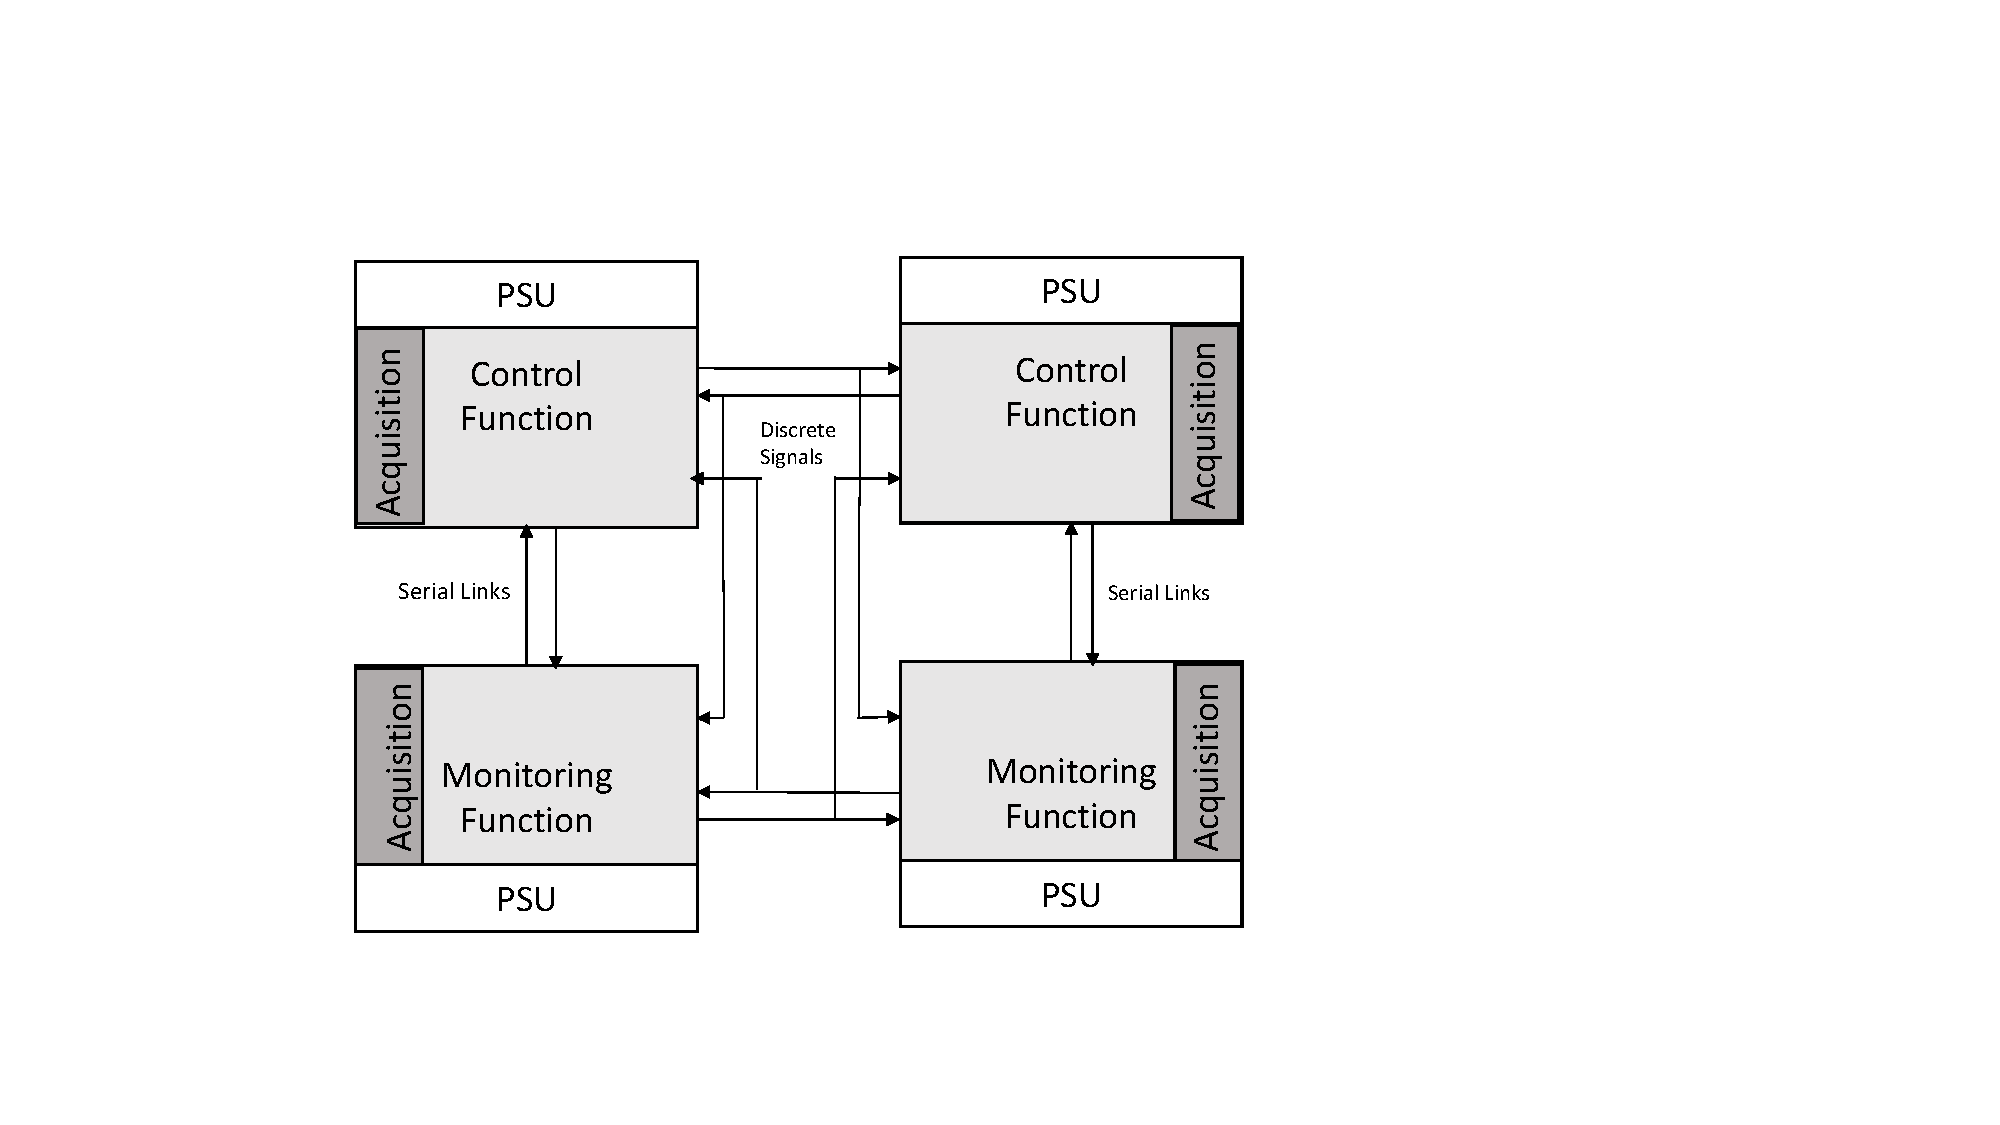
\includegraphics[width=\textwidth]{figures/BSCU.pdf}
\caption{BSCU Function Schematic from~\cite{a320ibiza}.}
\label{fig:BSCU_schematic}
\end{center}
\end{figure}

In the A320 system as shown in Figure~\ref{fig:BSCU_schematic} from~\cite{a320ibiza}, the BSCU comprises two channels, with each channel incorporating command and monitor lanes.  The command lane provides the active
control path to the system, whereas the monitor lane checks and enforces that
the command lane is operating within the expected envelope of performance. On
the detection of the first failure, the monitoring lane indicates a failure, and
control is passed to the other channel.  All processing of the system is
executed using a quasi-synchronous computational model. That is to say,
processing of each channel is quasi-synchronous with respect to one another,
and the channels themselves are also quasi-synchronous.

In the Ibiza incident, the root cause of the loss of normal and alternative
braking systems, was the Byzantine induced failure of both BSCU channels. The
failure was due to the sampling of the auto-brake mode control input panel
buttons. The auto-brake panel comprise three buttons, \texttt{LO}, \texttt{MED} and \texttt{MAX} that can
be used to select the corresponding auto-braking mode.  Momentarily pushing the
\texttt{LO} button selects the \texttt{LO} auto-braking mode. Pressing \texttt{LO} again de-selects the
auto-braking function, whereas pressing the \texttt{MED} or \texttt{MAX} buttons  selects the
corresponding automatic braking  modes. The state of the selected mode is
communicated to the crew by indicators for each mode that are illuminated when
the corresponding mode is active.

In the Airbus implementation, the buttons were sampled periodically by software
every 25ms. Given the asynchronous composition of the system, each processor
samples the button state relative to its own operating time-line. This
implementation is vulnerable to short button presses that are too short (< 25ms)
and therefore not consistently perceived by all of the sampling units as shown in figure \ref{fig:push_button_sampling}.
(Additional inter-lane mode agreement logic, to mitigate Byzantine sampling is
not implemented in the system~\footnote{Given that the command and monitor lanes
  are configured to be a fault-set, best practice would have implemented ingress
  agreement logic to prevent a fault external to the pair from disrupting the
  paired agreement.}.) Hence, the system failure occurred when the command and
monitoring lanes of both channels fell into disagreement, following the momentary 
selection of the \texttt{LO} auto-brake mode. The \texttt{LO} selection was only detected by one
of the lanes of each channel, hence the command and monitor mode disagreement
detection logic was erroneously stimulated . In the excursion, the disagreement
occurred on both channels simultaneously. Given that the system mode logic was
also event driven, there was no path to recovery. Pressing \texttt{LO} would be subject
to the same Byzantine vulnerability, and even if not Byzantine, the
incrementally edge driven mode selection logic would not recover into a
consistent state.

\begin{figure}
\begin{center}
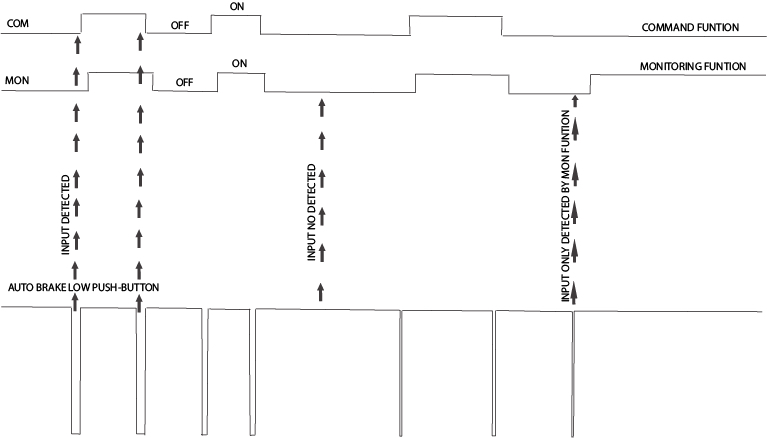
\includegraphics[width=0.85\textwidth]{figures/newtrace.jpg}
\caption{Oscilloscope chart of pressing times of AUTO/BRK LO vs. acquisition times of COM/MON functions}
\label{fig:push_button_sampling}
\end{center}
\end{figure}

 The design errors represent a failures uncovered by the traditional design assurance
 framework.  Given, the correct by construction synthesis focus, it is unlikely
 that our approach would allow such an implementation to be developed.  However,
 ensuring that the formal synthesis framework is sufficient to represent and
 explore such design vulnerabilities is a good test case for the ADSL formal
 tooling.  In addition to the agreement and mitigation if the Byzantine failure
 of the push button detection, the A320 Airbus brake system offers a good context
 to expand initial ADSL asynchronous exploration. For example, the system also
 requires a protocol to manage the channel in control, and additional logic and
 protocols to that communication is healthy.  From the incident report these
 details of the Airbus protocol implementations in these areas are not
 available. From the description it appears that the channel-in-control logic
 utilizes and asymmetric power-on timeout to yield a first-up channel in
 control. This may also leave the system vulnerable to assumptions of BSCU
 power-on order, and transient recovery strategies.  The protocols may also be
 vulnerable to failures of the inter-lane and inter-channel communication lines.
  Utilizing the provisions within the LIMA\ workbench, the long-term goal
of this case-study is to support the systematic exploration of candidate
protocols and fault models; yielding a better understanding how protocol
and communication architecture related design decisions impact core-system
properties.
  \subsubsection{Formal Model}




The formal model  of the  Wheel Brake System closely follows the structure  of  Figures 2.
However, to simplify the logic, and to reduce the size of the model, the
three buttons of the brake control panel are abstracted into a single button
that selects between manual and auto-mode operation.  The channel in control
is also simplified from the temporal first-up raced based selection, to a  fixed-priority scheme, where a pre-configured preferred channel remains in control
until it is faulted. Although simpler this model is sufficient to explore and demonstrate the byzantine failure vulnerability of the original system. 

The formal model starts with a top-level wbs atom that is used
to host all the system subcomponents. At the top level, three channels
are also implemented, two to convey the button status to each of the lanes,
and a third to convey the button state to the lane observer processes, that are used to host the properties that re to be formally investigated.
The   implementation of the lanes leverages and illustrates DSL\ provisions for parameterized replication.
 Using a map as shown below,  each lane is instantiated using with an assigned boolean  priority;  as described above   this priority arbitrates which lane is on control when the system is in full-up operational mode (i.e. no faults present).

\begin{lima}
 -- Declare two lanes
  laneIns <- mapM mkLane [True, False]  -- high/low priority
\end{lima}

 The lane implementation comprises two clocked periodic processes, one each for the  command and monitor  functions, together with an  an initialization  atom. At every period, the command and monitor sample the input from the button and toggle status of a boolean  operational model variable \textit{cautoMode},  on the detection of a rising button edge.  At each period, the update status of the \textit{cautoMod}e variable is shared with the local lane monitor.
 The DSL\ extract for this logic is shown below.



\begin{lima}

   cautoMode <== mux ((value bs ==. Const True) &&.
                       (value prevbs ==. Const False))
                      (not_ (value cautoMode))
                      (value cautoMode)
    writeChannel ctoIn (value framecount)  -- send 'framecount' to observer
    writeChannel ctmIn (value cautoMode)
      
\end{lima}
  The principal periodic process of the monitor atom is symmetrical to the periodic command atom. However, the monitor logic is extended with additional agreement counting logic, to monitor the agreement of the local and  command lane exchanged   \emph{cautoMode}  status. If disagreement persists   for three periods, the  monitor channel yields control to the other lane, by signaling  agreement failure.  

\begin{lima}
atom "wait_x_side_autoMode" $ do
      cond $ fullChannel ctmOut
      v <- readChannel ctmOut
      xSideAutoMode <== v
      probeP "monitor.XsideAutoMode" (value xSideAutoMode)

 atom "mon_agreement" $ do
      agreementFailureCount <==
        mux (value mautoMode /=. value xSideAutoMode)
            (Const one + value agreementFailureCount)
            (Const zero)
      -- cond $ value mautoMode /=. value xSideAutoMode
      -- incr agreementFailureCount

    atom "mon_agreement_count" $ do
      cond $ value agreementFailureCount ==. Const three
      agreementFailure <== Const True

\end{lima}

The representation of the WBS\ model in the DSL\ is very compact with the core logic only requiring about 150 lines of code.
 When contrasted with the approximately 12,000
lines of sally code, which the LIMA\ synthesizes,  this is a significant reduction. It may be argued, that without such a DSL and the associated synthesis, the industrial viability of sally alone may be challenging.

  
 Properties of interest  are simply asserted within any of the atoms as illustrated below. However, it should be noted that the variables used within the assert statements need to be within the atom scope.
 To simply model construction and instrumentation, it is recommended that variables significant to system properties are sent to a top-level observer process, that can provide a central point of property specification.  


\begin{lima}
 atom "mon_agreement" $ do
   agreementFailureCount <=  =
        mux (value mautoMode /=. value xSideAutoMode)
            (Const one + value agreementFailureCount)
            (Const zero)
   assert (pName pp "my assert")(value agreementFailureCount <=. Const three)
\end{lima}

In the Airbus braking example, no physical faults were actually present. Hence, in our initial model, we also omit a  fault model. However, the DSL\ framework ensures that the full state of the asynchronous interaction of the sampling and channel in control logic, will be explored within the synthesized  sally model. Therefore, the workbench is anticipated to uncover the system Byzantine failure as part of the formal model analysis.

As part of future work, we intend to augment the fault model
of the intra-lane and inter-lane, communication channels, and use the DSL\
and workbench to explore how such failures can impact the assumed system
level invariants,
and safety properties. We also intend to re-introduce the first up   leader
election protocol, which selects the initial lane in control. One again,
we envisage that this will demonstrate how the DSL\ and formal analysis workbench will support the systematic exploration of how
potential faults, and start-up timing variations can disrupt and impact
system safety properties and assumptions.  \   


%% \subsubsection{Verification}

%% \begin{figure}
%% \begin{center}
%% 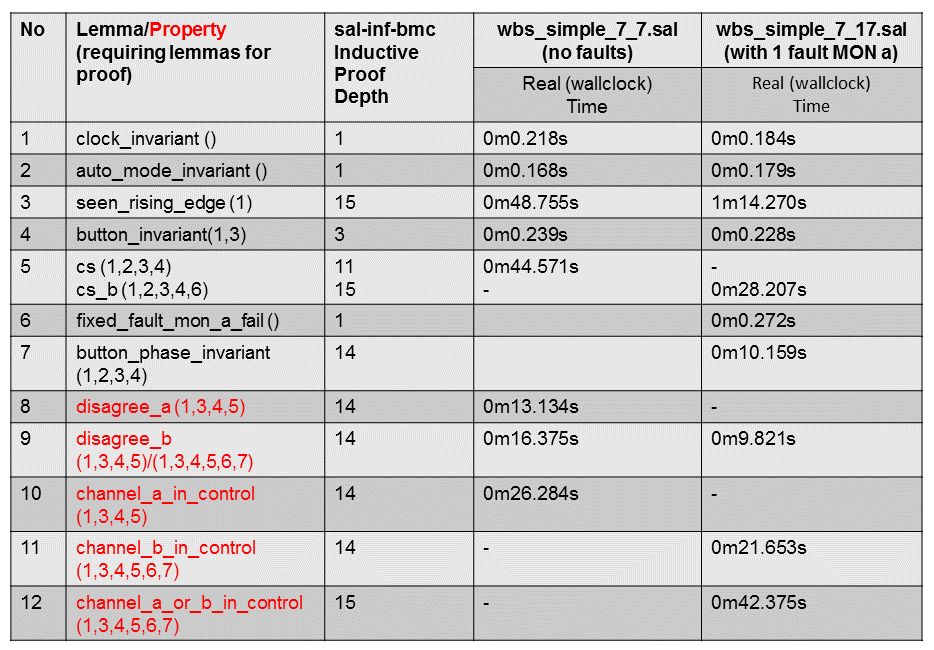
\includegraphics[width=1.0\textwidth]{figures/WBS_results}
%% \caption{WBS Proofs, Lemmas, Scalability Results and Performance}
%% \label{fig:WBS_results}
%% \end{center}
%% \end{figure}

%% Figure \ref{fig:WBS_results} summarizes the k-inductive proofs of the two code listings \ref{lst:wbssal1} and \ref{lst:wbssal2} and the set of lemmas that need to first proved before subsequently proving the desired properties of WBS listed in section \ref{subsubsec:ADSL_WBS_SAL}. We then also provide the scalability results with respect how much \emph{depth ('k' in k-induction)} is required to prove the lemmas/properties and also show timing/performance in terms of wall clock time.

%% The properties \emph{disagree\_a, disagree\_b, channel\_a\_in\_control} for code listing \ref{lst:wbssal1} and properties \emph{disagree\_b, channel\_b\_in\_control,channel\_a\_or\_b\_in\_control} for code listing \ref{lst:wbssal2} has already been described in section \ref{subsubsec:ADSL_WBS_SAL}. Next we describe the individual lemmas:

%% \begin{enumerate}

%% \item \emph{clock\_invariant} in lines $325-344,399$ of code listing \ref{lst:wbssal1}: This is a lemma that proves 4 things: (i) time is always non-negative or has value -1 indicating mutex (for exclusive operation on the calendar) (ii) time progresses montonously increasing i.e. the calendar processes each temporal event such that the next processed time is never less than the previous time (iii) mutexes on the calendar is processed atomically whereby if any task has the same value of -1 implies the the two tasks are identical and (iv) time is processed systematically so that all task clocks  for $com1$, $mon1$, $com2$ and $mon2$ are within the same period and their phase differences between the task clocks are properly advanced. \emph{Comment: This lemma is expected to be automatically generated from the ADSL}

%% \item \emph{auto\_mode\_invariant} in lines $354-360,401$ of code listing \ref{lst:wbssal1}: Ensures the \emph{initialization} of $com1$, $mon1$, $com2$ and $mon2$ i.e. com and mon across both channels a and b are properly initialized if the $button$ has not been pressed. \emph{This lemma is expected to be automatically generated from the ADSL} 

%% \item \emph{seen\_rising\_edge} in lines $366,402$ of code listing \ref{lst:wbssal1}: This lemma proves that if time has progressed greater than \emph{twice} the sampling period of $com1$, $mon1$, $com2$ and $mon2$, then the \emph{rising edge} of the push button of being pressed is guaranteed be detected by all of nodes $com1$, $mon1$, $com2$ and $mon2$. Alternatively if time is -1 (mutex) or had progressed to be less than the sampling period of $com1$, $mon1$, $com2$ and $mon2$, then the \emph{rising edge} of the push button of being pressed is guaranteed to NOT be detected by any of nodes $com1$, $mon1$, $com2$ and $mon2$. \emph{This lemma is expected to be manually specified within the ADSL} 

%% \item \emph{button\_invariant} in lines $347-351,400$ of code listing \ref{lst:wbssal1}: Proves that the button state variables are properly initialized. \emph{This lemma is expected to be automatically generated from the ADSL} 

%% \item \emph{cs} in lines $364,403$ of code listing \ref{lst:wbssal1}: This lemma proves that if time has progressed greater than \emph{twice} the sampling period of $com1$, $mon1$, $com2$ and $mon2$, then $com1$ mode selection must match $mon1$ and also $com2$ mode selection must match $mon2$ as sufficient time has elapsed for the two channels to both see the push button being pressed and hence \emph{seen\_rising\_edge} being detected. \emph{This lemma is expected to be manually specified within the ADSL} 

%% \item \emph{fixed\_fault\_mon\_a\_fail} in lines $522$ of code listing \ref{lst:wbssal2}: Directly based on the fault hypothesis. \emph{This lemma is expected to be automatically generated from the ADSL} 

%% \item \emph{cs\_b} in lines $456,512$ of code listing \ref{lst:wbssal2}: This lemma proves that if time has progressed greater than \emph{twice} the sampling period of $com2$ and $mon2$, then $com2$ mode selection must match $mon2$ as sufficient time has elapsed for the two channels to both see the push button being pressed and hence \emph{seen\_rising\_edge} being detected. \emph{This lemma is expected to be manually specified within the ADSL} 

%% \item \emph{button\_phase\_invariant} in lines $428-436,505$ of code listing \ref{lst:wbssal2}: The lemma ensures that time is processed systematically so that all task clocks  for $com1$, $mon1$, $com2$ and $mon2$ are within the same period and their phase differences between the task clocks are properly advanced and simultaneously ensuring these are done before the \emph{button} $period$ which is at a much slower rate. \emph{Comment: This lemma is expected to be automatically generated from the ADSL}

%% \end{enumerate}

%% As seen above, except for 3 lemmas (\emph{seen\_rising\_edge,cs,cs\_b}) which have to manually generated from ADSL, the rest of them can be automatically generated. Further the methodology to automatically deduce the \emph{depth} for k-induction (3rd column in figure \ref{fig:WBS_results}) must be investigated. Finally the dependencies or order of proving lemmas before proving the properties (listed in 2nd column in figure \ref{fig:WBS_results}) must also be investigated. \emph{These three issues listed must be resolved before AFFIRM workbench can guarantee that the necessary lemmas and k-induction proof of properties can automatically be synthesized}.  

%% \begin{figure}
%% \begin{center}
%% 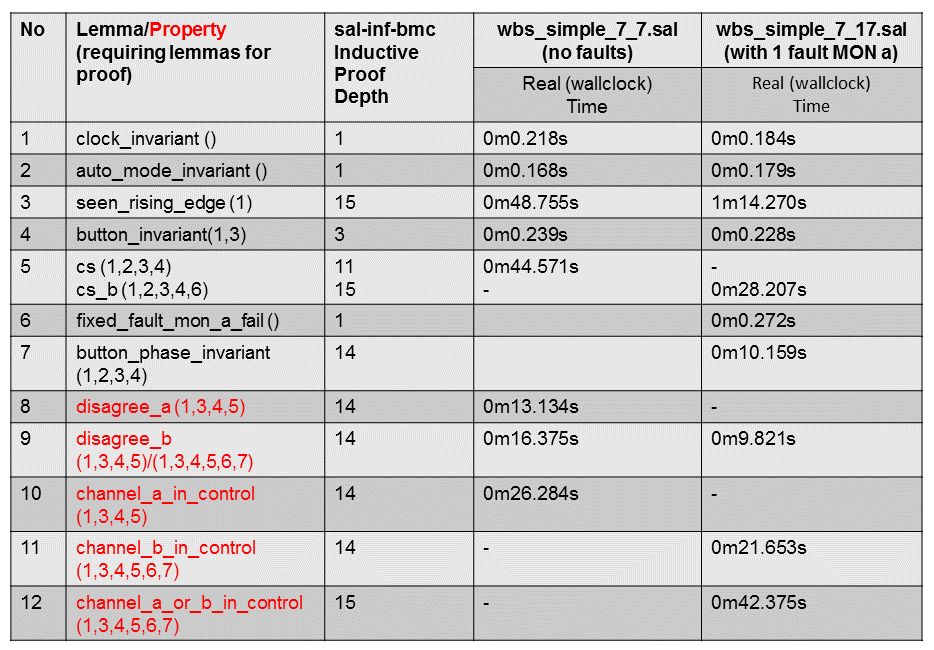
\includegraphics[width=1.0\textwidth]{figures/WBS_results}
%% \caption{WBS Proofs, Lemmas, Scalability Results and Performance}
%% \label{fig:WBS_results}
%% \end{center}
%% \end{figure}

%% Figure \ref{fig:WBS_results} summarizes the k-inductive proofs of the two code listings \ref{lst:wbssal1} and \ref{lst:wbssal2} and the set of lemmas that need to first proved before subsequently proving the desired properties of WBS listed in section \ref{subsubsec:ADSL_WBS_SAL}. We then also provide the scalability results with respect how much \emph{depth ('k' in k-induction)} is required to prove the lemmas/properties and also show timing/performance in terms of wall clock time.

%% The properties \emph{disagree\_a, disagree\_b, channel\_a\_in\_control} for code listing \ref{lst:wbssal1} and properties \emph{disagree\_b, channel\_b\_in\_control,channel\_a\_or\_b\_in\_control} for code listing \ref{lst:wbssal2} has already been described in section \ref{subsubsec:ADSL_WBS_SAL}. Next we describe the individual lemmas:

%% \begin{enumerate}

%% \item \emph{clock\_invariant} in lines $325-344,399$ of code listing \ref{lst:wbssal1}: This is a lemma that proves 4 things: (i) time is always non-negative or has value -1 indicating mutex (for exclusive operation on the calendar) (ii) time progresses montonously increasing i.e. the calendar processes each temporal event such that the next processed time is never less than the previous time (iii) mutexes on the calendar is processed atomically whereby if any task has the same value of -1 implies the the two tasks are identical and (iv) time is processed systematically so that all task clocks  for $com1$, $mon1$, $com2$ and $mon2$ are within the same period and their phase differences between the task clocks are properly advanced. \emph{Comment: This lemma is expected to be automatically generated from the ADSL}

%% \item \emph{auto\_mode\_invariant} in lines $354-360,401$ of code listing \ref{lst:wbssal1}: Ensures the \emph{initialization} of $com1$, $mon1$, $com2$ and $mon2$ i.e. com and mon across both channels a and b are properly initialized if the $button$ has not been pressed. \emph{This lemma is expected to be automatically generated from the ADSL} 

%% \item \emph{seen\_rising\_edge} in lines $366,402$ of code listing \ref{lst:wbssal1}: This lemma proves that if time has progressed greater than \emph{twice} the sampling period of $com1$, $mon1$, $com2$ and $mon2$, then the \emph{rising edge} of the push button of being pressed is guaranteed be detected by all of nodes $com1$, $mon1$, $com2$ and $mon2$. Alternatively if time is -1 (mutex) or had progressed to be less than the sampling period of $com1$, $mon1$, $com2$ and $mon2$, then the \emph{rising edge} of the push button of being pressed is guaranteed to NOT be detected by any of nodes $com1$, $mon1$, $com2$ and $mon2$. \emph{This lemma is expected to be manually specified within the ADSL} 

%% \item \emph{button\_invariant} in lines $347-351,400$ of code listing \ref{lst:wbssal1}: Proves that the button state variables are properly initialized. \emph{This lemma is expected to be automatically generated from the ADSL} 

%% \item \emph{cs} in lines $364,403$ of code listing \ref{lst:wbssal1}: This lemma proves that if time has progressed greater than \emph{twice} the sampling period of $com1$, $mon1$, $com2$ and $mon2$, then $com1$ mode selection must match $mon1$ and also $com2$ mode selection must match $mon2$ as sufficient time has elapsed for the two channels to both see the push button being pressed and hence \emph{seen\_rising\_edge} being detected. \emph{This lemma is expected to be manually specified within the ADSL} 

%% \item \emph{fixed\_fault\_mon\_a\_fail} in lines $522$ of code listing \ref{lst:wbssal2}: Directly based on the fault hypothesis. \emph{This lemma is expected to be automatically generated from the ADSL} 

%% \item \emph{cs\_b} in lines $456,512$ of code listing \ref{lst:wbssal2}: This lemma proves that if time has progressed greater than \emph{twice} the sampling period of $com2$ and $mon2$, then $com2$ mode selection must match $mon2$ as sufficient time has elapsed for the two channels to both see the push button being pressed and hence \emph{seen\_rising\_edge} being detected. \emph{This lemma is expected to be manually specified within the ADSL} 

%% \item \emph{button\_phase\_invariant} in lines $428-436,505$ of code listing \ref{lst:wbssal2}: The lemma ensures that time is processed systematically so that all task clocks  for $com1$, $mon1$, $com2$ and $mon2$ are within the same period and their phase differences between the task clocks are properly advanced and simultaneously ensuring these are done before the \emph{button} $period$ which is at a much slower rate. \emph{Comment: This lemma is expected to be automatically generated from the ADSL}

%% \end{enumerate}

%% As seen above, except for 3 lemmas (\emph{seen\_rising\_edge,cs,cs\_b}) which have to manually generated from ADSL, the rest of them can be automatically generated. Further the methodology to automatically deduce the \emph{depth} for k-induction (3rd column in figure \ref{fig:WBS_results}) must be investigated. Finally the dependencies or order of proving lemmas before proving the properties (listed in 2nd column in figure \ref{fig:WBS_results}) must also be investigated. \emph{These three issues listed must be resolved before AFFIRM workbench can guarantee that the necessary lemmas and k-induction proof of properties can automatically be synthesized}.  
